\documentclass[innermargin=10mm]{tikzposter}
\usepackage{enumitem}
\geometry{paperwidth=197cm,paperheight=100cm}
\usepackage{url}

\usepackage{alltt}

\newcommand{\inst}[1]{\hspace{2pt}$^{\mbox{\normalsize#1}}$\hspace{-7pt}}
\newcommand{\instlist}[1]{\hspace{1pt}$^{#1}$}

\title{
  \begin{minipage}{\textwidth}
    \centering
    Analyzing rasters, vectors and time series using new Python interfaces in GRASS GIS 7
    \bigskip
  \end{minipage}
}
\author{
V\'{a}clav Petr\'{a}\v{s}\inst{1},
Anna Petr\'{a}\v{s}ov\'{a}\inst{1},
Yann Chemin\inst{2},
Pietro Zambelli\inst{3},
Martin Landa\inst{4},
S\"{o}ren Gebbert\inst{5},
Markus Neteler\inst{6}, and
Peter L\"{o}we\inst{7}
}
\institute{
\large
\instlist{1}North Carolina State University, Raleigh, USA (wenzeslaus@gmail.com, vpetras@ncsu.edu),
\instlist{2}International Water Management Institute, Pelawatta, Sri Lanka,
\instlist{3}EURAC Research, Institute for Renewable Energy, Bolzano/Bozen, Italy,
\instlist{4}Faculty of Civil Engineering, Czech Technical University in Prague, Czech Republic,
\instlist{5}Th\"{u}nen Institute of Climate-Smart Agriculture, Braunschweig, Germany,
\instlist{6}Research and Innovation Centre, Fondazione Edmund Mach, San Michele all'Adige, Italy,
\instlist{7}German National Library for Science and Technology, Hanover, Germany
}
% \titlegraphic{}

\pdfinfo{
   /Author (Vaclav Petras, Anna Petrasova, Yann Chemin, Pietro Zambelli, Martin Landa, Soeren Gebbert, Markus Neteler, and Peter Loewe)
   /Title  (Analyzing rasters, vectors and time series using new Python interfaces in GRASS GIS 7)
%    /Subject (ensuring reproducibility of scientific geospatial computing - this is from testing poster)
   /Keywords (GIS, API, algorithms, open science, reproducibility)
}

\definecolor{textcolor}{HTML}{000000}

\definecolor{titleTextColor}{HTML}{2E652E}


\definecolorpalette{sampleColorPalette} {
  \definecolor{colorOne}{HTML}{419041}
  % \definecolor{colorTwo}{HTML}{cccccc}
  \definecolor{colorTwo}{HTML}{dddddd}
  \definecolor{colorThree}{HTML}{F1B52D}
  % \definecolor{colorThree}{HTML}{EFA126}
}


\usetheme{Rays}
\usecolorstyle[colorPalette=sampleColorPalette]{Britain}
\useblockstyle{Default} % Basic
% \usecolorpalette{e}

\makeatletter
\renewcommand\TP@maketitle{%
    \begin{minipage}{0.12\linewidth}
       \centering
       
       \newcommand{\logowidth}{0.17\textwidth}
       \newcommand{\logovspace}{\vspace{3ex}}
       \newcommand{\logohspace}{\hspace{1ex}}
       
       % TODO: get other logos
       
\includegraphics[width=\logowidth]{ncstate}
       \logohspace
       
\includegraphics[width=\logowidth]{iwmi}

       \logovspace

       
\includegraphics[width=\logowidth]{ncstate}
       \logohspace
       
\includegraphics[width=\logowidth]{ctu_prague}
       \logohspace
       
\includegraphics[width=\logowidth]{ncstate}

       \logovspace

       
\includegraphics[width=\logowidth]{fem_cri}
       \logohspace
       
\includegraphics[width=\logowidth]{ncstate}
    \end{minipage}%
    \hfill
   \begin{minipage}{0.74\linewidth}
        \centering
        \color{titlefgcolor}
        {\textcolor{titleTextColor}{\textsf{\textbf{{\fontsize{85}{60}\selectfont \@title}}}}  \par}
        \vspace*{1em}
        {\huge \@author \par}
        \vspace*{1em}
        {\LARGE \@institute}
    \end{minipage}%
    \hfill
    \begin{minipage}{0.12\linewidth}
       \centering
       
\includegraphics[width=0.35\textwidth]{grass}\\
       \Large \textbf{\textsf{GRASS GIS}}
    \end{minipage}
}
\setlength{\TP@visibletextwidth}{\textwidth-3\TP@innermargin}
\setlength{\TP@visibletextheight}{\textheight-3\TP@innermargin}

\makeatother

\setlength{\parskip}{1ex}

\graphicspath{{images/}{logos/}{qrcodes/}{listings/}}

% listings package does not work well with the tikzposter class,
% so we need to include PDFs with code generated separately

\newcommand{\partitle}[1]{\bigskip \textbf{#1}\\[1ex]}
\newcommand{\parinlinetitle}[1]{\bigskip \textbf{#1}\ }
\newcommand{\textfontsize}{\LARGE}

% GRASS module
\newcommand{\gmodule}[1]{\emph{#1}}

\newcommand{\rafun}[1]{\texttt{#1()}}

% GRASS Python package
\newcommand{\pkg}[1]{\emph{#1}}

\begin{document}
\maketitle[width=0.95\textwidth]



\begin{columns}

%%%%%%%%%%%%%%%%%%%%%%%%%%%%%%%%%%%%%%%%%%%%%%%%%%%%%%%%%%%%%%%%%%%%%
%%%%%%%%%%%%%%%%%%%%%%%%%%%%%%%%%%%%%%%%%%%%%%%%%%%%%%%%%%%%%%%%%%%%%
%%%%%%%%%%%%%%%%%%%%%%%%%%%%%%%%%%%%%%%%%%%%%%%%%%%%%%%%%%%%%%%%%%%%%
%%%%%%%%%%%%%%%%%%%%%%%%%%%%%%%%%%%%%%%%%%%%%%%%%%%%%%%%%%%%%%%%%%%%%
\column{0.25}

% Abstract from http://meetingorganizer.copernicus.org/EGU2015/EGU2015-8142.pdf
%
% GRASS GIS 7 is a free and open source GIS software developed and used by many scientists (Neteler et al., 2012).
% While some users of GRASS GIS prefer its graphical user interface, significant part of the scientific community
% takes advantage of various scripting and programing interfaces offered by GRASS GIS to develop new models and
% algorithms. Here we will present different interfaces added to GRASS GIS 7 and available in Python, a popular
% programming language and environment in geosciences. These Python interfaces are designed to satisfy the needs
% of scientists and programmers under various circumstances.
% 
% PyGRASS (Zambelli et al., 2013) is a new object-oriented interface to GRASS GIS modules and libraries.
% The GRASS GIS libraries are implemented in C to ensure maximum performance and the PyGRASS interface
% provides an intuitive, pythonic access to their functionality. GRASS GIS Python scripting library is another way of
% accessing GRASS GIS modules. It combines the simplicity of Bash and the efficiency of the Python syntax. When
% full access to all low-level and advanced functions and structures from GRASS GIS library is required, Python
% programmers can use an interface based on the Python ctypes package. Ctypes interface provides complete, direct
% access to all functionality as it would be available to C programmers.
%
% GRASS GIS provides specialized Python library for managing and analyzing spatio-temporal data (Gebbert and
% Pebesma, 2014). The temporal library introduces space time datasets representing time series of raster, 3D raster
% or vector maps and allows users to combine various spatio-temporal operations including queries, aggregation,
% sampling or the analysis of spatio-temporal topology.
% 
% We will also discuss the advantages of implementing scientific algorithm as a GRASS GIS module and we will
% show how to write such module in Python. To facilitate the development of the module, GRASS GIS provides
% a Python library for testing (Petras and Gebbert, 2014) which helps researchers to ensure the robustness of the
% algorithm, correctness of the results in edge cases as well as the detection of changes in results due to new
% development. For all modules GRASS GIS automatically creates standardized command line and graphical user
% interfaces and documentation. Finally, we will show how GRASS GIS can be used together with powerful Python
% tools such as the NumPy package and the IPython Notebook.

% TODO: the two blocks below are just taken from testing poster

%%%%%%%%%%%%%%%%%%%%%%%%%%%%%%%%%%%%%%%%%%%%%%%%%%%%%%%%%%%%%%%%%%%%%
\block{Highlights}{
% \setlength{\parskip}{1em}
\textfontsize
% \begin{itemize}
\renewcommand{\item}{\par\vspace{0.8ex}}
\item GRASS GIS is a platform for geospatial computations.
\item The framework supports code maintenance which results in long term preservation of algorithms.
}

%%%%%%%%%%%%%%%%%%%%%%%%%%%%%%%%%%%%%%%%%%%%%%%%%%%%%%%%%%%%%%%%%%%%%
\block{Description}{
% \textfontsize
\Large
\newcommand{\intropartitle}[1]{\parinlinetitle{#1}}
% \setlength{\parskip}{1em}

\intropartitle{Motivation}
GRASS GIS \cite{Neteler2012}, a free and open source GIS, is used by many scientists directly or through other projects such as R or QGIS to perform geoprocessing tasks.
Thus, a large number of scientific geospatial computations depend on quality and correct functionality of GRASS GIS.
Automatic functionality testing is therefore necessary to ensure software reliability.

\intropartitle{Unique features}
We present a testing framework for GRASS GIS which addresses different needs of GRASS GIS and geospatial software in general.
It tests GRASS tools (referred to as GRASS modules) and
examines outputs including large raster and vector maps as well as temporal datasets.
Furthermore, it enables to test all levels of GRASS GIS architecture including C and Python application programming interface and GRASS modules invoked as subprocesses.

\intropartitle{Audience}
Since GRASS GIS is used as a platform for development of geospatial algorithms and models,
the testing framework allows not only to test GRASS GIS core functionality but also tools developed by scientists as a part of their research.

\intropartitle{Scientific impact}
}

\block{More information}{
\newcommand{\qrcodewidth}{1\linewidth}
\hspace{-0.02\linewidth}
\begin{tabular}{lll}
\begin{minipage}{0.1\linewidth}

\includegraphics[height=\qrcodewidth]{grass_osgeo_org}
\end{minipage}
\begin{minipage}{0.27\linewidth}
GRASS GIS website
\end{minipage}
&
\begin{minipage}{0.1\linewidth}

\includegraphics[height=\qrcodewidth]{python_doc}
\end{minipage}
\begin{minipage}{0.45\linewidth}
GRASS GIS Python libraries documentation
\end{minipage}
\\
% http://grass.osgeo.org/
\url{grass.osgeo.org}
&
% http://grass.osgeo.org/grass71/manuals/libpython/
\url{grass.osgeo.org/grass71/manuals/libpython}
\end{tabular}

% qrcode -t EPS -o grass-user.eps "http://lists.osgeo.org/listinfo/grass-user"
% epstopdf grass-user.eps
% rm grass-user.eps

}

%%%%%%%%%%%%%%%%%%%%%%%%%%%%%%%%%%%%%%%%%%%%%%%%%%%%%%%%%%%%%%%%%%%%%
%%%%%%%%%%%%%%%%%%%%%%%%%%%%%%%%%%%%%%%%%%%%%%%%%%%%%%%%%%%%%%%%%%%%%
%%%%%%%%%%%%%%%%%%%%%%%%%%%%%%%%%%%%%%%%%%%%%%%%%%%%%%%%%%%%%%%%%%%%%
%%%%%%%%%%%%%%%%%%%%%%%%%%%%%%%%%%%%%%%%%%%%%%%%%%%%%%%%%%%%%%%%%%%%%
\column{0.25}


\block{GRASS Scripting library interface to GRASS GIS modules}{

The same applies to \pkg{grass.pygrass} syntax:

\includegraphics[width=\linewidth, clip, trim=0 0 0 0]{script_doc_syntax}

}

%%%%%%%%%%%%%%%%%%%%%%%%%%%%%%%%%%%%%%%%%%%%%%%%%%%%%%%%%%%%%%%%%%%%%
\block{PyGRASS interface to GRASS GIS modules}{

The same applies to \pkg{grass.pygrass} syntax:

\includegraphics[width=\linewidth, clip, trim=0 0 0 0]{pygrass_doc_syntax}

}

%%%%%%%%%%%%%%%%%%%%%%%%%%%%%%%%%%%%%%%%%%%%%%%%%%%%%%%%%%%%%%%%%%%%%
\block{Using documentation for GRASS GIS modules}{

Documentation of GRASS GIS modules usually use Bash syntax for examples:

\begin{alltt}
r.neighbors input=elevation output=elevation\_smooth method=median -c
\end{alltt}

This can be easily rewritten to \pkg{grass.script} syntax:

\includegraphics[width=\linewidth, clip, trim=0 0 0 0]{script_doc_syntax}

The same applies to \pkg{grass.script} syntax:

\includegraphics[width=\linewidth, clip, trim=0 0 0 0]{pygrass_doc_syntax}

}

%%%%%%%%%%%%%%%%%%%%%%%%%%%%%%%%%%%%%%%%%%%%%%%%%%%%%%%%%%%%%%%%%%%%%
\block{\pkg{ctypes} interface to C libraries}{

}

%%%%%%%%%%%%%%%%%%%%%%%%%%%%%%%%%%%%%%%%%%%%%%%%%%%%%%%%%%%%%%%%%%%%%
\block{Using NumPy}{

}

%%%%%%%%%%%%%%%%%%%%%%%%%%%%%%%%%%%%%%%%%%%%%%%%%%%%%%%%%%%%%%%%%%%%%
\block{Using IPython Notebook}{

}

%%%%%%%%%%%%%%%%%%%%%%%%%%%%%%%%%%%%%%%%%%%%%%%%%%%%%%%%%%%%%%%%%%%%%
%%%%%%%%%%%%%%%%%%%%%%%%%%%%%%%%%%%%%%%%%%%%%%%%%%%%%%%%%%%%%%%%%%%%%
%%%%%%%%%%%%%%%%%%%%%%%%%%%%%%%%%%%%%%%%%%%%%%%%%%%%%%%%%%%%%%%%%%%%%
%%%%%%%%%%%%%%%%%%%%%%%%%%%%%%%%%%%%%%%%%%%%%%%%%%%%%%%%%%%%%%%%%%%%%
\column{0.25}

%%%%%%%%%%%%%%%%%%%%%%%%%%%%%%%%%%%%%%%%%%%%%%%%%%%%%%%%%%%%%%%%%%%%%
\block{Automatic creation of GUI and CLI}{

\includegraphics[width=\linewidth, clip, trim=0 0 0 0]{grass_module}

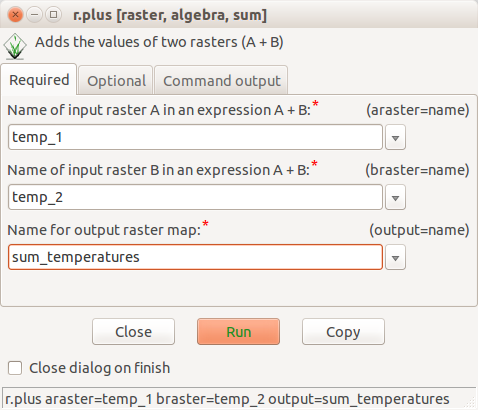
\includegraphics[width=0.5\linewidth, clip, trim=0 0 0 0]{grass_module_gui}
\includegraphics[width=0.5\linewidth, clip, trim=0 0 0 0]{grass_module_cli}

}

%%%%%%%%%%%%%%%%%%%%%%%%%%%%%%%%%%%%%%%%%%%%%%%%%%%%%%%%%%%%%%%%%%%%%
\block{PyGRASS interface to C libraries}{

}

%%%%%%%%%%%%%%%%%%%%%%%%%%%%%%%%%%%%%%%%%%%%%%%%%%%%%%%%%%%%%%%%%%%%%
\block{Python script versus GRASS GIS module}{
and running code from IDE
}


%%%%%%%%%%%%%%%%%%%%%%%%%%%%%%%%%%%%%%%%%%%%%%%%%%%%%%%%%%%%%%%%%%%%%
%%%%%%%%%%%%%%%%%%%%%%%%%%%%%%%%%%%%%%%%%%%%%%%%%%%%%%%%%%%%%%%%%%%%%
%%%%%%%%%%%%%%%%%%%%%%%%%%%%%%%%%%%%%%%%%%%%%%%%%%%%%%%%%%%%%%%%%%%%%
%%%%%%%%%%%%%%%%%%%%%%%%%%%%%%%%%%%%%%%%%%%%%%%%%%%%%%%%%%%%%%%%%%%%%
\column{0.25}

%%%%%%%%%%%%%%%%%%%%%%%%%%%%%%%%%%%%%%%%%%%%%%%%%%%%%%%%%%%%%%%%%%%%%
\block{Temporal framework}{

}

%%%%%%%%%%%%%%%%%%%%%%%%%%%%%%%%%%%%%%%%%%%%%%%%%%%%%%%%%%%%%%%%%%%%%
\block{Testing the code}{

}

%%%%%%%%%%%%%%%%%%%%%%%%%%%%%%%%%%%%%%%%%%%%%%%%%%%%%%%%%%%%%%%%%%%%%
\block{GRASS GIS Addons}{
The GRASS GIS Addons ensures long-term preservation of the code.
Well maintained modules in Addons can be moved to GRASS GIS itself.
}

%%%%%%%%%%%%%%%%%%%%%%%%%%%%%%%%%%%%%%%%%%%%%%%%%%%%%%%%%%%%%%%%%%%%%
\block{Alternatives to Python}{
GRASS GIS modules are command line tools, so they can be used in shell scripting (e.g. Bash)
and as subprocesses virtually any language as long as proper environment is set.

The GRASS GIS library has a C API which is often used to create GRASS modules in C and C++.

GRASS GIS modules can be used in R using \pkg{rgrass7} package.
}

%%%%%%%%%%%%%%%%%%%%%%%%%%%%%%%%%%%%%%%%%%%%%%%%%%%%%%%%%%%%%%%%%%%%%
\block{Acknowledgements}{
\begin{tabular}{cp{0.75\linewidth}}
\raisebox{-.4\height}{

\includegraphics[width=0.2\linewidth]{osgeo}
}
& GRASS GIS is a OSGeo project. OSGeo provides infrastructure for websites and source code management.
\\
\raisebox{-.8\height}{

\includegraphics[width=0.2\linewidth]{google}
}
& Initial development of \pkg{pygrass} and \pkg{gunittest} packages was done during Google Summer of Code.
\end{tabular}
}


%%%%%%%%%%%%%%%%%%%%%%%%%%%%%%%%%%%%%%%%%%%%%%%%%%%%%%%%%%%%%%%%%%%%%
\block{References}{

% disable the title
\renewcommand{\section}[2]{}
\begin{thebibliography}{9}

\bibitem{Neteler2012}
  Neteler, M., Bowman, M. H., Landa, M., Metz, M., 2012.
  \emph{GRASS GIS: A multi-purpose open source GIS.}
  Environmental Modelling \& Software, 31(0), 124-130.

\bibitem{Gebbert2014}
  Gebbert, S., Pebesma, E., 2014. A temporal GIS for field based environmental modeling. Environmental
  Modelling \& Software 53, 1-12.

\bibitem{Petras2014}
  Petras, V., Gebbert, S., 2014. Testing framework for GRASS GIS: ensuring reproducibility of scientific
  geospatial computing. Poster presented at: AGU Fall Meeting, December 15-19, 2014, San Francisco, USA.

\bibitem{Zambelli2013}
  Zambelli, P., Gebbert, S., Ciolli, M., 2013. Pygrass: An Object Oriented Python Application Programming
  Interface (API) for Geographic Resources Analysis Support System (GRASS) Geographic Information System
  (GIS). ISPRS International Journal of Geo-Information 2, 201-219.

\end{thebibliography}
}

\end{columns}
\end{document}